\documentclass[a4paper,11pt,exos]{nsi} % COMPILE WITH DRAFT
\usepackage{pifont}
\usepackage{fontawesome5}

\pagestyle{empty}

\begin{document}
\classe{\premiere spé}
\titre{Défi 1}
\maketitle

\begin{center}
    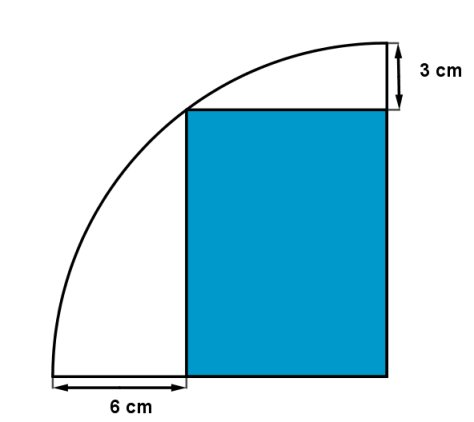
\includegraphics[width=8cm]{Aire.jpg}
\end{center}

Quelle est l'aire du rectangle ?\\

\vspace*{3cm}


\maketitle

\begin{center}
    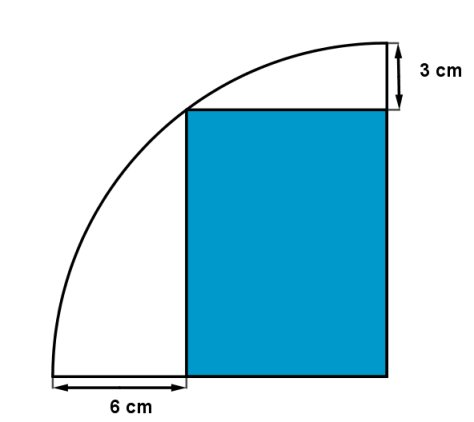
\includegraphics[width=8cm]{Aire.jpg}
\end{center}

Quelle est l'aire du rectangle ?
\end{document}